\documentclass[letterpaper,11pt]{article}

\oddsidemargin 0.0in
\evensidemargin 0.0in
\textwidth 6.5in


\usepackage[tocbib,bibnewpage]{apacite}
\usepackage{graphics}
\usepackage{amsmath}
\usepackage{indentfirst}
\usepackage{tabularx}
\usepackage{graphicx}
\usepackage{url}
\usepackage{appendix}
\usepackage{verbatim}
\usepackage{lscape}
\usepackage{rotating}

\usepackage{ifthen}
\newboolean{internal}
\setboolean{internal}{true} %===== Internal Document =====%


\DeclareMathOperator{\var}{var}
\DeclareMathOperator{\cov}{cov}

\usepackage{Sweave}
\begin{document}

\title{\texttt{irutils}: An R Package for Institutional Research}
\author{Jason M. Bryer\\
\small{}jbryer@expcelsior.edu\\
Excelsior College}
\date{\today}

\maketitle

\abstract{This document specifies the functions available in the \texttt{irutils} package. This package is designed to accomony the \textit{Introduction to R and \LaTeX} document. The package provides many functions useful for typical reporting requirements of Institutional Research offices.
\ \\ \ \\
\noindent Keywords: \textit{institutional research, database, higher education, ipeds}}


\section{Introduction}

The \texttt{irutils} package is hosted at \url{http://github.com/jbryer/irutils}. The \texttt{devtools} \cite{devtools} package provides functions to assist in R package development including a function to install directly from github. The \texttt{install\_github} will install the latest development version of the \texttt{irutils} package.

\begin{Schunk}
\begin{Sinput}
> library(devtools)
> install_github('devtools', 'jbryer')
\end{Sinput}
\end{Schunk}

The currently available functions are:
\begin{Schunk}
\begin{Sinput}
> library(irutils)
> ls('package:irutils')
\end{Sinput}
\begin{Soutput}
 [1] "adjustedTableLaTeX"       "cacheQuery"              
 [3] "cohortRetention"          "cohortSummary"           
 [5] "cohortSummaryLaTeX"       "createLocalRepos"        
 [7] "execQuery"                "fySummary"               
 [9] "fySummaryLaTeX"           "geocode.google"          
[11] "geocode.ips"              "geocode.yahoo"           
[13] "geolite.delete"           "geolite.load"            
[15] "geolite.update"           "geolite.version"         
[17] "getAge"                   "getAgeGroups"            
[19] "getAgeGroupsIPEDS"        "getParameters"           
[21] "getQueries"               "getQuery"                
[23] "getQueryDesc"             "getSQLRepos"             
[25] "local.available.packages" "local.install.packages"  
[27] "plotBarchartTable"        "plotCohortRetention"     
[29] "plotHeatmapTable"         "plotPersistence"         
[31] "plotRetention"            "plotRetentionOverall"    
[33] "retention"                "retentionSummary"        
[35] "retentionSummaryLaTeX"    "saveIPEDStoDB"           
[37] "setSQLRepos"              "updateLocalRepos"        
\end{Soutput}
\end{Schunk}



\section{Database Access}

For many Institutional Research offices the institutions student information system (SIS) is the most common source of data. Since virtually all SIS systems are backed by a database, extracting data requires extracting data using queries. Typically the language used to extract data is called structured query language (SQL) regardless if the database is provided by Oracle, Microsoft, or an open source options such as MySQL and PostgreSQL. There are a number of functions in this package that will faciliate extracting data from these databases directly into R.

The database access functions provide an interface to a directory of SQL scripts. SQL scripts are simply a plain text file containing the query. The directory containing these files can be determined or set using the \texttt{getSQLRepos} and \texttt{setSQLRepos} functions, repsectively. 

\begin{Schunk}
\begin{Sinput}
> getSQLRepos()
\end{Sinput}
\begin{Soutput}
[1] "O:/Resources/R/library/irutils/data"
\end{Soutput}
\end{Schunk}

By convention, all SQL files must use a \texttt{.sql} file extension. The \texttt{getQueries} function will return a list of all the queries available in the current reposistory.

\begin{Schunk}
\begin{Sinput}
> getQueries()
\end{Sinput}
\begin{Soutput}
[1] "TestQuery"
\end{Soutput}
\end{Schunk}

The \texttt{getQueryDesc} and \texttt{getParameters} functions will provide some details about the query in question. In particular, the latter will return the parameters that are required for the query to execute.

\begin{Schunk}
\begin{Sinput}
> getQueryDesc('TestQuery')
\end{Sinput}
\begin{Soutput}
[1] ""
\end{Soutput}
\begin{Sinput}
> getParameters('TestQuery')
\end{Sinput}
\begin{Soutput}
[1] "ContactID"
\end{Soutput}
\end{Schunk}

There are two functions available for executing the query. The \texttt{execQuery} will execute the query and return a data frame. The \texttt{cacheQuery} however, will first look in the specified directory (by default the \texttt{dir} parameter is set to \texttt{getwd()}) for a CSV file that matches the currently request query. That is, the file name (which is returned when this function is executed) is built using a combination of the query name and parameters to uniquely identify it. This is useful when using Sweave and \LaTeX for document preparation where the function may be executed multiple times but the data does not change. It is considerably faster to read data from a flat file then it is to query the database each time.

\subsection{Creating Your Own Query}

To create your own query, simply place the SQL statement in its own text file ending with \texttt{.sql}. Comments can be placed in the file using the \texttt{\#} symbol. Placing informative comments at the beginning of the file will be useful since the \texttt{getQueryDesc} function will return these comments to the user. Parameters can be placed anywhere in the file and must be enclosed within colons (i.e. the : character). Additionally, parameter names must begin with a letter, contain only letters and numbers, and cannot have any spaces.

\begin{figure}[h]
\begin{center}
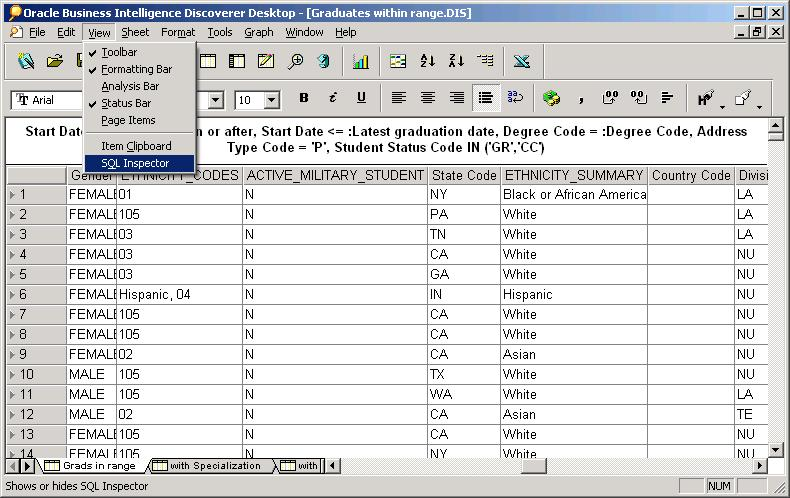
\includegraphics{DiscovererMenu}
\caption{Beginning 72-Month Completion Rates by Military Status}
\label{fig:discoverer}
\end{center}
\end{figure}



\section{Visualizing Likert Response Items}

\begin{Schunk}
\begin{Sinput}
> data(pisa)
> items28 = pisa[,substr(names(pisa), 1,5) == 'ST24Q']
> names(items28) = c("I read only if I have to.",
+    "Reading is one of my favorite hobbies.",
+    "I like talking about books with other people.",
+    "I find it hard to finish books.",
+    "I feel happy if I receive a book as a present.",
+    "For me, reading is a waste of time.",
+    "I enjoy going to a bookstore or a library.",
+    "I read only to get information that I need.",
+    "I cannot sit still and read for more than a few minutes.",
+    "I like to express my opinions about books I have read.",
+    "I like to exchange books with my friends")
> for(i in 1:ncol(items28)) {
+ 	items28[,i] = factor(items28[,i], levels=1:4, 
+ 		labels=c('Strongly disagree', 'Disagree', 'Agree', 'Strongly Agree'),
+ 		ordered=TRUE)
+ }
\end{Sinput}
\end{Schunk}

\begin{figure}
\begin{center}
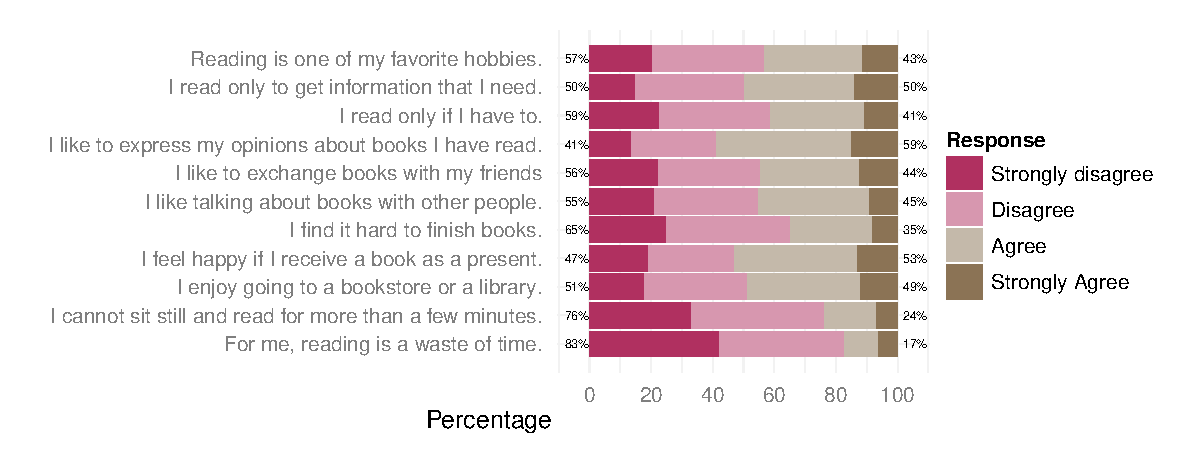
\includegraphics{irutils-PISAItem28BarchartTable1}
\caption{Barchart Table Graphic}
\label{fig:PISAItem28BarchartTable1}
\end{center}
\end{figure}

\begin{figure}
\begin{center}
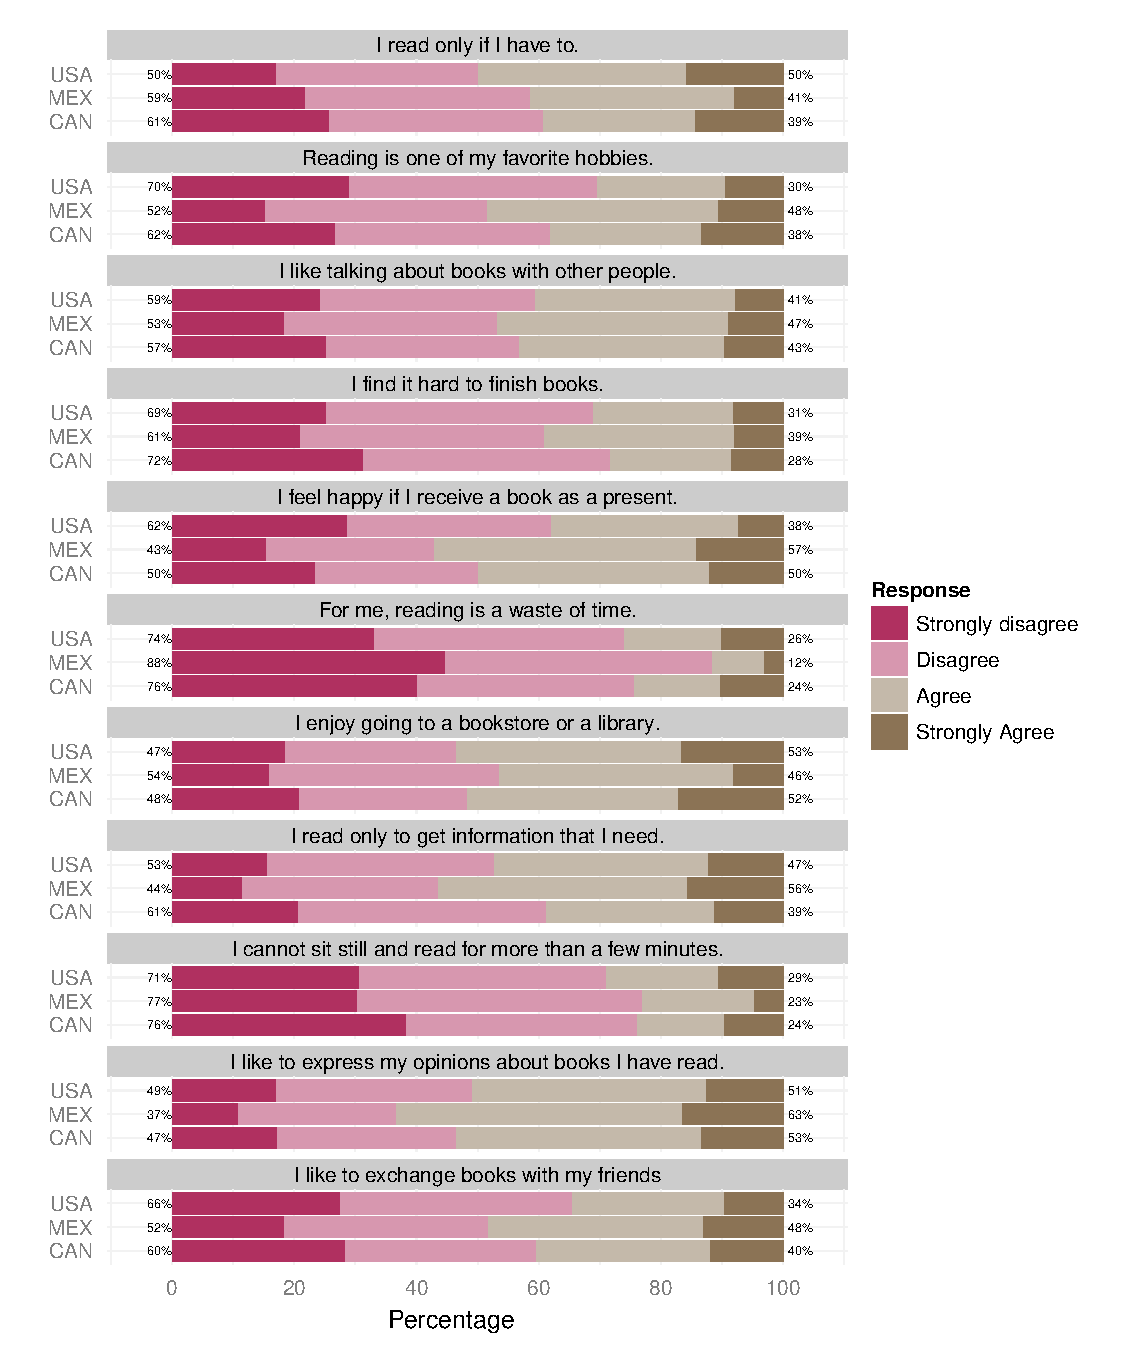
\includegraphics{irutils-PISAItem28BarchartTable2}
\caption{Barchart Table Graphic Grouped by Country}
\label{fig:PISAItem28BarchartTable2}
\end{center}
\end{figure}


\section{Retention and Completion Rates}


\clearpage
\bibliographystyle{apacite}
\bibliography{Bibliography}


\end{document}
